\documentclass{standalone}

\usepackage{tikz}
\usetikzlibrary{shapes, snakes, patterns, arrows}
\usetikzlibrary{calc}

\begin{document}

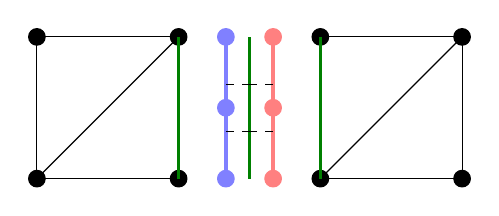
\begin{tikzpicture}[scale=0.60]
      % Minus
  \draw[black] (0, 0) rectangle (3, 3);
  \draw[black] (0, 0) -- (3, 3);
  \node[mark size=3pt, color=black] at (0, 0) {\pgfuseplotmark{*}};
  \node[mark size=3pt, color=black] at (3, 0) {\pgfuseplotmark{*}};
  \node[mark size=3pt, color=black] at (0, 3) {\pgfuseplotmark{*}};
  \node[mark size=3pt, color=black] at (3, 3) {\pgfuseplotmark{*}};
    
  \draw[black] (6, 0) rectangle (9, 3);
  \draw[black] (6, 0) -- (9, 3);
  \node[mark size=3pt, color=black] at (6, 0) {\pgfuseplotmark{*}};
  \node[mark size=3pt, color=black] at (9, 0) {\pgfuseplotmark{*}};
  \node[mark size=3pt, color=black] at (6, 3) {\pgfuseplotmark{*}};
  \node[mark size=3pt, color=black] at (9, 3) {\pgfuseplotmark{*}};

  \draw[green!50!black, very thick] (3, 0) -- (3, 3);
  \draw[green!50!black, very thick] (6, 0) -- (6, 3);
  \draw[green!50!black, very thick] (4.5, 0) -- (4.5, 3);
 % \node[green!50!black, below] at (4.5, 0) {$\Gamma$};

  \draw[white!50!blue, very thick] (4, 0) -- (4, 3);
  \node[mark size=3pt, color=white!50!blue] at (4, 0) {\pgfuseplotmark{*}};
  \node[mark size=3pt, color=white!50!blue] at (4, 3) {\pgfuseplotmark{*}};
  \node[mark size=3pt, color=white!50!blue] at (4, 1.5) {\pgfuseplotmark{*}};
  \draw[thin, black, dashed] (4, 1) -- (4.5, 1);
  \draw[thin, black, dashed] (4, 2) -- (4.5, 2);
%  \node[white!50!blue, above] at (4, 3) {$\hat{\Gamma}_h$};

  \draw[white!50!red, very thick] (5, 0) -- (5, 3);
  \node[mark size=3pt, color=white!50!red] at (5, 0) {\pgfuseplotmark{*}};
  \node[mark size=3pt, color=white!50!red] at (5, 3) {\pgfuseplotmark{*}};
  \node[mark size=3pt, color=white!50!red] at (5, 1.5) {\pgfuseplotmark{*}};
  \draw[thin, black, dashed] (5, 1) -- (4.5, 1);
  \draw[thin, black, dashed] (5, 2) -- (4.5, 2);
%  \node[white!50!red, above] at (5, 3) {${\Gamma}_h$};
\end{tikzpicture}

\end{document}
